\documentclass{article}

% content/resources/templates/preamble.tex
\usepackage[margin=0.6in]{geometry}
\author{Milav Dabgar}
\usepackage{amsmath,amssymb,amsthm}
\usepackage{booktabs}
\usepackage{multirow}
\usepackage{xcolor}
\usepackage{tcolorbox}
\tcbuselibrary{breakable,skins}
\usepackage[colorlinks=true,linkcolor=blue]{hyperref}
\usepackage{titlesec}
\usepackage{enumitem}
\usepackage{tikz}
\usepackage{pgfplots}
\usepackage{circuitikz}
\usepackage[version=4]{mhchem}
\usepackage{longtable}
\usepackage{array}
\usepackage{float}
\usepackage{caption}
\usepackage{listings}

\lstset{
  basicstyle=\small\ttfamily,
  breaklines=true,
  breakatwhitespace=false,
  postbreak=\mbox{\textcolor{red}{$\hookrightarrow$}\space},
  float=false,
  numbers=left,
  numberstyle=\tiny\color{gray},
  numbersep=10pt,
  xleftmargin=2em,
  keywordstyle=\color{blue},
  commentstyle=\color{green!60!black},
  stringstyle=\color{purple},
  backgroundcolor=\color{gray!5},
  showstringspaces=false,
  tabsize=2,
  captionpos=b,
  keepspaces=true,
  columns=flexible
}

\pgfplotsset{compat=1.18}
\usetikzlibrary{shapes,arrows,positioning,calc,patterns,decorations.pathmorphing,decorations.markings,arrows.meta}

% Color scheme
\definecolor{headcolor}{RGB}{0,102,204}
\definecolor{keycolor}{RGB}{220,20,60}
\definecolor{solutioncolor}{RGB}{34,139,34}
\definecolor{mnemoniccolor}{RGB}{148,0,211}
\definecolor{codecolor}{RGB}{0,0,100}

% Spacing
\setlength{\parskip}{3pt}
\setlist[itemize]{nosep}
\setlist[enumerate]{nosep}

% Title formatting
\titleformat{\section}{\Large\bfseries\color{headcolor}}{\thesection}{1em}{}
\titleformat{\subsection}{\large\bfseries\color{headcolor}}{\thesubsection}{1em}{}

% Pandoc tightlist compatibility
\providecommand{\tightlist}{%
  \setlength{\itemsep}{0pt}\setlength{\parskip}{0pt}}

% Pandoc longtable compatibility
\newcounter{none}
\def\thenone{}


% content/resources/templates/english-boxes.tex

% Custom environments
\newtcolorbox{solutionbox}{
 breakable,
 enhanced,
 colback=solutioncolor!5!white,
 colframe=solutioncolor!75!black,
 fonttitle=\bfseries,
 title=Solution
}

\newtcolorbox{solutionboxnobreak}{
 colback=solutioncolor!5!white,
 colframe=solutioncolor!75!black,
 fonttitle=\bfseries,
 title=Solution
}

\newtcolorbox{keyformula}{
 breakable,
 enhanced,
 colback=keycolor!5!white,
 colframe=keycolor!75!black,
 fonttitle=\bfseries,
 title=Key Formula
}

\newtcolorbox{mnemonicboxenv}{
 breakable,
 enhanced,
 colback=mnemoniccolor!5!white,
 colframe=mnemoniccolor!75!black,
 fonttitle=\bfseries,
 title=Mnemonic
}

\newcommand{\mnemonicbox}[1]{%
  \begin{mnemonicboxenv}
    #1
  \end{mnemonicboxenv}
}


% Custom commands for GTU solutions
% This file defines semantic commands for consistent formatting

% Question command with automatic formatting
\newcommand{\question}[2]{%
  \section*{Question #1}%
  \textbf{#2}%
}

% OR question variant
\newcommand{\questionor}[2]{%
  \section*{Question #1 OR}%
  \textbf{#2}%
}

% Proper table environment with caption
\newenvironment{answertable}[1]{%
  \begin{table}[htbp]
  \centering
  \caption{#1}
}{%
  \end{table}
}

% Proper figure environment for diagrams
\newenvironment{answerdiagram}[1]{%
  \begin{figure}[htbp]
  \centering
  \caption{#1}
}{%
  \end{figure}
}

% Semantic markup for key terms
\newcommand{\keyword}[1]{\textbf{#1}}
\newcommand{\code}[1]{\texttt{#1}}
\newcommand{\classname}[1]{\texttt{#1}}
\newcommand{\methodname}[1]{\texttt{#1}}

% Proper quotation marks
\newcommand{\mnemonic}[1]{``#1''}


\title{Fundamentals of Blockchain (4361603) - Summer 2024 Solution}
\date{May 18, 2024}

\begin{document}
\maketitle

\questionmarks{1(a)}{3}{Explain benefits of using distributed ledger systems.}

\begin{solutionbox}
\textbf{Answer}:

\begin{center}
\captionof{table}{Benefits of Distributed Ledger Systems}
\begin{tabulary}{\linewidth}{|L|L|}
\hline
\textbf{Benefit} & \textbf{Description} \\ \hline
\keyword{Transparency} & All participants can view transaction history \\ \hline
\keyword{Security} & Cryptographic protection against tampering \\ \hline
\keyword{Decentralization} & No single point of failure or control \\ \hline
\keyword{Immutability} & Records cannot be altered once confirmed \\ \hline
\end{tabulary}
\end{center}

\begin{mnemonicbox}
\mnemonic{T-S-D-I: Transparent, Secure, Decentralized, Immutable}
\end{mnemonicbox}
\end{solutionbox}

\questionmarks{1(b)}{4}{Define: 1) Blockchain 2) Distributed systems}

\begin{solutionbox}
\textbf{Answer}:

\begin{center}
\captionof{table}{Key Definitions}
\begin{tabulary}{\linewidth}{|L|L|}
\hline
\textbf{Term} & \textbf{Definition} \\ \hline
\textbf{Blockchain} & A chain of blocks containing transaction data, linked using cryptographic hashes \\ \hline
\textbf{Distributed Systems} & Network of independent computers working together as a single system \\ \hline
\end{tabulary}
\end{center}

\textbf{Key Features}:

\begin{itemize}
    \item \textbf{Blockchain}: Uses hash pointers, consensus mechanisms, and merkle trees
    \item \textbf{Distributed Systems}: Fault tolerance, scalability, and resource sharing
\end{itemize}

\begin{mnemonicbox}
\mnemonic{Chain-Hash-Consensus for Blockchain, Network-Independent-Together for Distributed}
\end{mnemonicbox}
\end{solutionbox}

\questionmarks{1(c)}{7}{Illustrate CAP theorem with the help of Blockchain network.}

\begin{solutionbox}
\textbf{Answer}:

\begin{center}
\captionof{table}{CAP Theorem Components}
\begin{tabulary}{\linewidth}{|L|L|L|}
\hline
\textbf{Property} & \textbf{Description} & \textbf{Blockchain Context} \\ \hline
\keyword{Consistency} & All nodes see same data & All nodes have identical ledger \\ \hline
\keyword{Availability} & System remains operational & Network stays accessible \\ \hline
\keyword{Partition Tolerance} & Works despite network failures & Continues during node disconnections \\ \hline
\end{tabulary}
\end{center}

\textbf{Diagram:}

\begin{center}
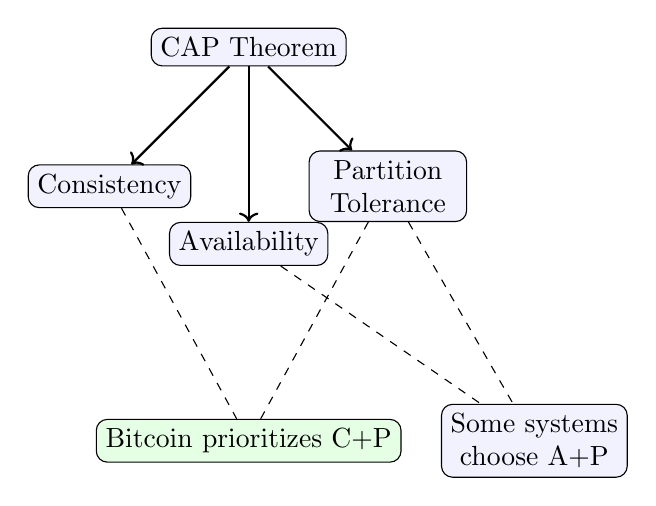
\begin{tikzpicture}[node distance=2.5cm, auto,
    gtu block/.style={rectangle, draw, rounded corners, align=center, fill=blue!5, minimum width=2cm},
    gtu arrow/.style={->, thick}]

    \node [gtu block] (cap) {CAP Theorem};
    \node [gtu block, below left of=cap] (cons) {Consistency};
    \node [gtu block, below of=cap] (avail) {Availability};
    \node [gtu block, below right of=cap] (part) {Partition\\Tolerance};

    \draw [gtu arrow] (cap) -- (cons);
    \draw [gtu arrow] (cap) -- (avail);
    \draw [gtu arrow] (cap) -- (part);
    
    \node [gtu block, below of=avail, fill=green!10] (btc) {Bitcoin prioritizes C+P};
    \draw [dashed] (cons) -- (btc);
    \draw [dashed] (part) -- (btc);
    
    \node [gtu block, right=0.5cm of btc] (others) {Some systems\\choose A+P};
    \draw [dashed] (avail) -- (others);
    \draw [dashed] (part) -- (others);

\end{tikzpicture}
\captionof{figure}{CAP Theorem in Blockchain}
\end{center}

\textbf{Key Points}:

\begin{itemize}
    \item \textbf{Trade-off}: Can only achieve 2 out of 3 properties simultaneously
    \item \textbf{Blockchain Choice}: Most blockchains choose Consistency + Partition Tolerance
    \item \textbf{Example}: Bitcoin may become temporarily unavailable but maintains consistency
\end{itemize}

\begin{mnemonicbox}
\mnemonic{CAP-2-out-of-3: Choose Any 2 Properties out of 3}
\end{mnemonicbox}
\end{solutionbox}

\questionmarks{1(c) OR}{7}{List and explain applications of blockchain network.}

\begin{solutionbox}
\textbf{Answer}:

\begin{center}
\captionof{table}{Blockchain Applications}
\begin{tabulary}{\linewidth}{|L|L|L|}
\hline
\textbf{Application} & \textbf{Description} & \textbf{Example} \\ \hline
\keyword{Cryptocurrency} & Digital money transactions & Bitcoin, Ethereum \\ \hline
\keyword{Supply Chain} & Track products from origin & Walmart food tracing \\ \hline
\keyword{Healthcare} & Secure patient records & Medical data sharing \\ \hline
\keyword{Voting} & Transparent elections & Estonia e-voting \\ \hline
\keyword{Real Estate} & Property ownership records & Land registries \\ \hline
\end{tabulary}
\end{center}

\textbf{Key Benefits}:

\begin{itemize}
    \item \textbf{Transparency}: All transactions visible to participants
    \item \textbf{Security}: Cryptographic protection against fraud
    \item \textbf{Efficiency}: Reduced intermediaries and costs
\end{itemize}

\begin{mnemonicbox}
\mnemonic{C-S-H-V-R: Crypto, Supply, Health, Vote, Real estate}
\end{mnemonicbox}
\end{solutionbox}

\questionmarks{2(a)}{3}{Define and explain a permissionless blockchain in detail.}

\begin{solutionbox}
\textbf{Answer}:

\textbf{Definition}: A blockchain where anyone can participate without requiring permission from a central authority.

\begin{center}
\captionof{table}{Permissionless Blockchain Features}
\begin{tabulary}{\linewidth}{|L|L|}
\hline
\textbf{Feature} & \textbf{Description} \\ \hline
\keyword{Open Access} & Anyone can join and participate \\ \hline
\keyword{Public Verification} & All transactions are publicly verifiable \\ \hline
\keyword{Decentralized} & No central controlling authority \\ \hline
\end{tabulary}
\end{center}

\textbf{Key Characteristics}:

\begin{itemize}
    \item \textbf{Consensus}: Uses proof-of-work or proof-of-stake
    \item \textbf{Examples}: Bitcoin, Ethereum mainnet
\end{itemize}

\begin{mnemonicbox}
\mnemonic{OPD: Open-Public-Decentralized}
\end{mnemonicbox}
\end{solutionbox}

\questionmarks{2(b)}{4}{Draw a figure and provide a brief explanation of a data structure of a blockchain.}

\begin{solutionbox}
\textbf{Answer}:

\textbf{Diagram: Blockchain Data Structure}

\begin{center}
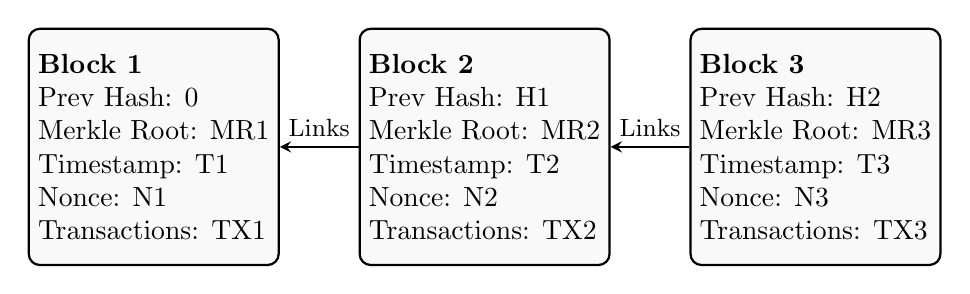
\begin{tikzpicture}[gtu block/.style={rectangle, draw, thick, rounded corners, minimum width=3cm, minimum height=3cm, align=left, fill=gray!5},
                    gtu arrow/.style={->, thick, >=stealth}]

    \node [gtu block] (b1) {\textbf{Block 1}\\Prev Hash: 0\\Merkle Root: MR1\\Timestamp: T1\\Nonce: N1\\Transactions: TX1};
    \node [gtu block, right=1.0cm of b1] (b2) {\textbf{Block 2}\\Prev Hash: H1\\Merkle Root: MR2\\Timestamp: T2\\Nonce: N2\\Transactions: TX2};
    \node [gtu block, right=1.0cm of b2] (b3) {\textbf{Block 3}\\Prev Hash: H2\\Merkle Root: MR3\\Timestamp: T3\\Nonce: N3\\Transactions: TX3};
    
    \draw [gtu arrow] (b2.west) -- node[above, font=\small] {Links} (b1.east);
    \draw [gtu arrow] (b3.west) -- node[above, font=\small] {Links} (b2.east);

\end{tikzpicture}
\captionof{figure}{Blockchain Data Structure}
\end{center}

\textbf{Key Components}:

\begin{itemize}
    \item \textbf{Previous Hash}: Links blocks together creating chain
    \item \textbf{Merkle Root}: Summary of all transactions in block
    \item \textbf{Timestamp}: When block was created
    \item \textbf{Nonce}: Number used once for proof-of-work
\end{itemize}

\begin{mnemonicbox}
\mnemonic{P-M-T-N: Previous, Merkle, Time, Nonce}
\end{mnemonicbox}
\end{solutionbox}

\questionmarks{2(c)}{7}{Explain the core components of blockchain with suitable diagrams.}

\begin{solutionbox}
\textbf{Answer}:

\begin{center}
\captionof{table}{Core Components of Blockchain}
\begin{tabulary}{\linewidth}{|L|L|L|}
\hline
\textbf{Component} & \textbf{Function} & \textbf{Purpose} \\ \hline
\keyword{Blocks} & Data containers & Store transaction information \\ \hline
\keyword{Hash Functions} & Create digital fingerprints & Ensure data integrity \\ \hline
\keyword{Merkle Trees} & Transaction summaries & Efficient verification \\ \hline
\keyword{Consensus Mechanism} & Agreement protocol & Validate new blocks \\ \hline
\keyword{Digital Signatures} & Identity verification & Authenticate transactions \\ \hline
\end{tabulary}
\end{center}

\textbf{Diagram: Merkle Tree Structure}

\begin{center}
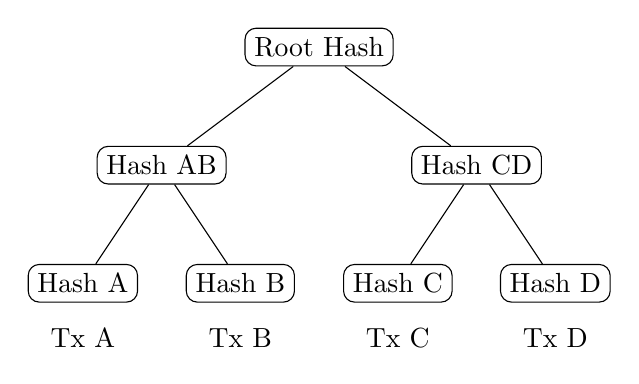
\begin{tikzpicture}[level distance=1.5cm,
  level 1/.style={sibling distance=4cm},
  level 2/.style={sibling distance=2cm},
  level 3/.style={sibling distance=1cm},
  gtu node/.style={rectangle, draw, rounded corners, align=center, fill=white}]

  \node [gtu node] {Root Hash}
    child {node [gtu node] {Hash AB}
      child {node [gtu node] (HashA) {Hash A}}
      child {node [gtu node] (HashB) {Hash B}}
    }
    child {node [gtu node] {Hash CD}
      child {node [gtu node] (HashC) {Hash C}}
      child {node [gtu node] (HashD) {Hash D}}
    };
    
    \node [below=0.2cm of HashA] {Tx A};
    \node [below=0.2cm of HashB] {Tx B};
    \node [below=0.2cm of HashC] {Tx C};
    \node [below=0.2cm of HashD] {Tx D};
\end{tikzpicture}
\captionof{figure}{Merkle Tree Structure}
\end{center}

\textbf{Key Points}:

\begin{itemize}
    \item \textbf{Immutability}: Hash functions make tampering detectable
    \item \textbf{Efficiency}: Merkle trees allow fast verification
    \item \textbf{Decentralization}: Consensus mechanisms eliminate central authority
\end{itemize}

\begin{mnemonicbox}
\mnemonic{B-H-M-C-D: Blocks, Hash, Merkle, Consensus, Digital}
\end{mnemonicbox}
\end{solutionbox}

\questionmarks{2(a) OR}{3}{Define and explain permissioned blockchain in detail.}

\begin{solutionbox}
\textbf{Answer}:

\textbf{Definition}: A blockchain where participation requires explicit permission from a governing authority.

\begin{center}
\captionof{table}{Permissioned Blockchain Features}
\begin{tabulary}{\linewidth}{|L|L|}
\hline
\textbf{Feature} & \textbf{Description} \\ \hline
\keyword{Restricted Access} & Only authorized users can participate \\ \hline
\keyword{Private Network} & Controlled membership \\ \hline
\keyword{Centralized Control} & Governing body manages permissions \\ \hline
\end{tabulary}
\end{center}

\textbf{Key Characteristics}:

\begin{itemize}
    \item \textbf{Privacy}: Enhanced confidentiality for sensitive data
    \item \textbf{Performance}: Faster transactions due to fewer validators
    \item \textbf{Examples}: Hyperledger Fabric, R3 Corda
\end{itemize}

\begin{mnemonicbox}
\mnemonic{RPC: Restricted-Private-Centralized}
\end{mnemonicbox}
\end{solutionbox}

\questionmarks{2(b) OR}{4}{Explain types of wallets in the context of blockchain. Also discuss the factors to be considered while selecting wallet for the specific need.}

\begin{solutionbox}
\textbf{Answer}:

\begin{center}
\captionof{table}{Types of Blockchain Wallets}
\begin{tabulary}{\linewidth}{|L|L|L|}
\hline
\textbf{Wallet Type} & \textbf{Description} & \textbf{Security Level} \\ \hline
\keyword{Hot Wallets} & Connected to internet & Medium \\ \hline
\keyword{Cold Wallets} & Offline storage & High \\ \hline
\keyword{Hardware Wallets} & Physical devices & Very High \\ \hline
\keyword{Paper Wallets} & Printed keys & High (if stored safely) \\ \hline
\end{tabulary}
\end{center}

\textbf{Selection Factors}:

\begin{itemize}
    \item \textbf{Security Requirements}: Higher value needs better security
    \item \textbf{Frequency of Use}: Regular use favors hot wallets
    \item \textbf{Technical Expertise}: Simple wallets for beginners
\end{itemize}

\begin{mnemonicbox}
\mnemonic{H-C-H-P: Hot, Cold, Hardware, Paper}
\end{mnemonicbox}
\end{solutionbox}

\questionmarks{2(c) OR}{7}{Explain sidechain in detail with suitable diagrams.}

\begin{solutionbox}
\textbf{Answer}:

\textbf{Definition}: A separate blockchain that is attached to a parent blockchain using a two-way peg.

\textbf{Diagram: Sidechain Architecture}

\begin{center}
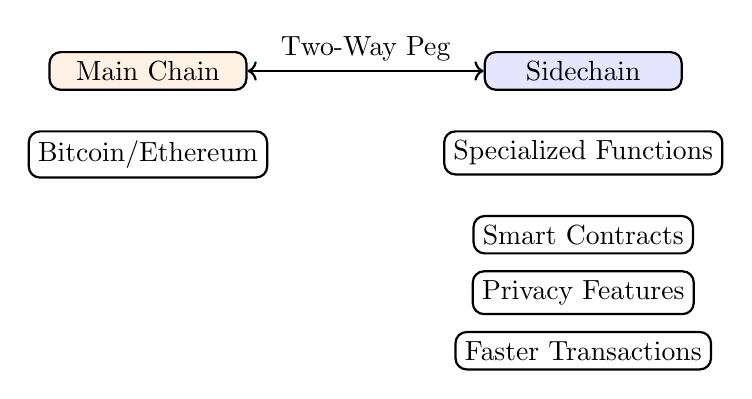
\begin{tikzpicture}[node distance=2.5cm, auto,
    gtu block/.style={rectangle, draw, thick, rounded corners, minimum width=2.5cm, align=center},
    gtu arrow/.style={->, thick}]

    \node [gtu block, fill=orange!10] (main) {Main Chain};
    \node [gtu block, below=0.5cm of main] (btc) {Bitcoin/Ethereum};
    
    \node [gtu block, right=3cm of main, fill=blue!10] (side) {Sidechain};
    \node [gtu block, below=0.5cm of side] (func) {Specialized Functions};
    
    \node [gtu block, below=0.5cm of func] (smart) {Smart Contracts};
    \node [gtu block, below=0.2cm of smart] (priv) {Privacy Features};
    \node [gtu block, below=0.2cm of priv] (fast) {Faster Transactions};
    
    \path (main) -- node[auto] (peg) {Two-Way Peg} (side);
    \draw [gtu arrow, <->] (main) -- (side);

\end{tikzpicture}
\captionof{figure}{Sidechain Architecture}
\end{center}

\begin{center}
\captionof{table}{Sidechain Benefits}
\begin{tabulary}{\linewidth}{|L|L|}
\hline
\textbf{Benefit} & \textbf{Description} \\ \hline
\keyword{Scalability} & Reduces load on main chain \\ \hline
\keyword{Experimentation} & Test new features safely \\ \hline
\keyword{Specialized Functions} & Custom applications \\ \hline
\keyword{Interoperability} & Connect different blockchains \\ \hline
\end{tabulary}
\end{center}

\textbf{Key Mechanisms}:

\begin{itemize}
    \item \textbf{Two-Way Peg}: Allows asset transfer between chains
    \item \textbf{SPV Proofs}: Simplified payment verification
    \item \textbf{Federated Control}: Multiple parties manage transfers
\end{itemize}

\begin{mnemonicbox}
\mnemonic{S-E-S-I: Scalability, Experimentation, Specialized, Interoperability}
\end{mnemonicbox}
\end{solutionbox}

\questionmarks{3(a)}{3}{With respect to transaction in a blockchain network, define the terms "Confirmation" and "Finality".}

\begin{solutionbox}
\textbf{Answer}:

\begin{center}
\captionof{table}{Transaction States}
\begin{tabulary}{\linewidth}{|L|L|}
\hline
\textbf{Term} & \textbf{Definition} \\ \hline
\keyword{Confirmation} & Number of blocks built on top of transaction block \\ \hline
\keyword{Finality} & Point where transaction becomes irreversible \\ \hline
\end{tabulary}
\end{center}

\textbf{Key Points}:

\begin{itemize}
    \item \textbf{Confirmation Count}: More confirmations = higher security
    \item \textbf{Bitcoin Standard}: 6 confirmations for high-value transactions
    \item \textbf{Finality Types}: Probabilistic (Bitcoin) vs Absolute (some PoS systems)
\end{itemize}

\begin{mnemonicbox}
\mnemonic{Count-Blocks-Security for Confirmation, Irreversible-Point for Finality}
\end{mnemonicbox}
\end{solutionbox}

\questionmarks{3(b)}{4}{Differentiate Proof of Work and Proof of Stake.}

\begin{solutionbox}
\textbf{Answer}:

\begin{center}
\captionof{table}{PoW vs PoS Comparison}
\begin{tabulary}{\linewidth}{|L|L|L|}
\hline
\textbf{Aspect} & \textbf{Proof of Work (PoW)} & \textbf{Proof of Stake (PoS)} \\ \hline
\textbf{Resource} & Computational power & Stake ownership \\ \hline
\textbf{Energy Use} & High & Low \\ \hline
\textbf{Security} & Hash rate dependent & Stake dependent \\ \hline
\textbf{Rewards} & Mining rewards & Staking rewards \\ \hline
\textbf{Examples} & Bitcoin, Ethereum (old) & Ethereum 2.0, Cardano \\ \hline
\end{tabulary}
\end{center}

\textbf{Key Differences}:

\begin{itemize}
    \item \textbf{Mechanism}: PoW uses mining, PoS uses validators
    \item \textbf{Environmental Impact}: PoS is more eco-friendly
    \item \textbf{Barriers to Entry}: PoS requires initial stake, PoW needs hardware
\end{itemize}

\begin{mnemonicbox}
\mnemonic{Work-vs-Stake: Computational Work vs Financial Stake}
\end{mnemonicbox}
\end{solutionbox}

\questionmarks{3(c)}{7}{With respect to blockchain network, explain 51\% attack.}

\begin{solutionbox}
\textbf{Answer}:

\textbf{Definition}: An attack where a single entity controls more than 50\% of the network's mining power or stake.

\textbf{Diagram: 51\% Attack Scenario}

\begin{center}
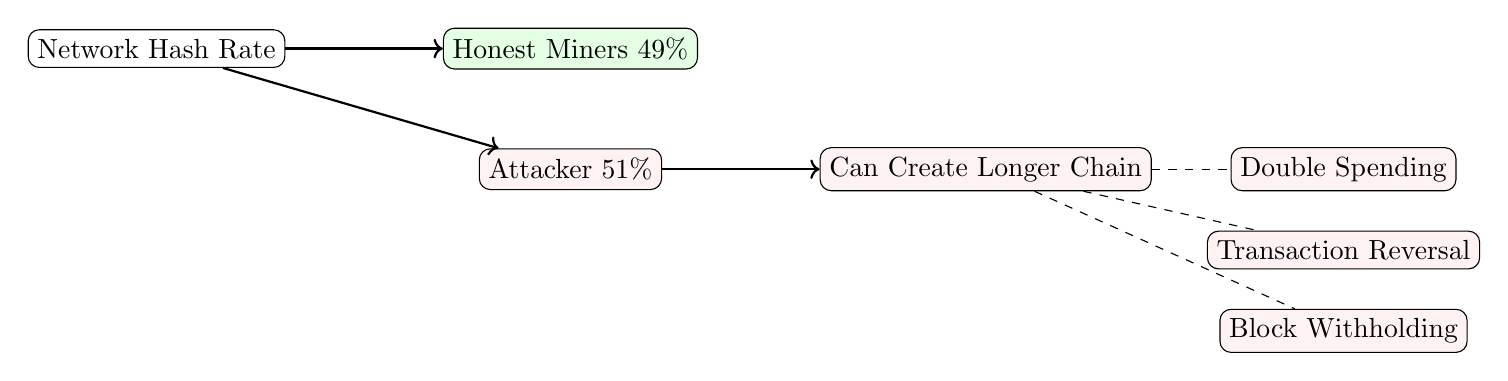
\begin{tikzpicture}[node distance=2cm, auto,
    gtu block/.style={rectangle, draw, rounded corners, align=center, fill=red!5},
    gtu arrow/.style={->, thick}]

    \node [gtu block, fill=white] (hash) {Network Hash Rate};
    \node [gtu block, right=2cm of hash, fill=green!10] (honest) {Honest Miners 49\%};
    \node [gtu block, below=1cm of honest] (attacker) {Attacker 51\%};
    
    \draw [gtu arrow] (hash) -- (honest);
    \draw [gtu arrow] (hash) -- (attacker);
    
    \node [gtu block, right=2cm of attacker] (longer) {Can Create Longer Chain};
    \draw [gtu arrow] (attacker) -- (longer);
    
    \node [gtu block, right=1cm of longer] (double) {Double Spending};
    \node [gtu block, below=0.5cm of double] (reversal) {Transaction Reversal};
    \node [gtu block, below=0.5cm of reversal] (withhold) {Block Withholding};
    
    \draw [dashed] (longer) -- (double);
    \draw [dashed] (longer) -- (reversal);
    \draw [dashed] (longer) -- (withhold);

\end{tikzpicture}
\captionof{figure}{51\% Attack Scenario}
\end{center}

\begin{center}
\captionof{table}{Attack Capabilities and Limitations}
\begin{tabulary}{\linewidth}{|L|L|}
\hline
\textbf{Can Do} & \textbf{Cannot Do} \\ \hline
Double spend own coins & Steal others' coins \\ \hline
Reverse recent transactions & Create coins from nothing \\ \hline
Block specific transactions & Change consensus rules \\ \hline
Fork the blockchain & Access private keys \\ \hline
\end{tabulary}
\end{center}

\textbf{Prevention Measures}:

\begin{itemize}
    \item \textbf{Diversified Mining}: Encourage multiple mining pools
    \item \textbf{Checkpoint Systems}: Periodic finality markers
    \item \textbf{Economic Incentives}: Make attacks unprofitable
\end{itemize}

\textbf{Impact}:

\begin{itemize}
    \item \textbf{Network Disruption}: Temporary service interruption
    \item \textbf{Economic Loss}: Reduced trust and value
    \item \textbf{Recovery}: Network usually recovers after attack ends
\end{itemize}

\begin{mnemonicbox}
\mnemonic{Majority-Control-Attack: 51\% = Majority Control = Attack Power}
\end{mnemonicbox}
\end{solutionbox}

\questionmarks{3(a) OR}{3}{Define the terms "Hard fork" and "Soft fork"}

\begin{solutionbox}
\textbf{Answer}:

\begin{center}
\captionof{table}{Fork Types}
\begin{tabulary}{\linewidth}{|L|L|L|}
\hline
\textbf{Fork Type} & \textbf{Definition} & \textbf{Compatibility} \\ \hline
\keyword{Hard Fork} & Non-backward compatible protocol change & Not compatible \\ \hline
\keyword{Soft Fork} & Backward compatible protocol change & Compatible \\ \hline
\end{tabulary}
\end{center}

\textbf{Key Characteristics}:

\begin{itemize}
    \item \textbf{Hard Fork}: Creates new blockchain branch, requires all nodes to upgrade
    \item \textbf{Soft Fork}: Tightens rules, old nodes can still operate
\end{itemize}

\textbf{Examples}:

\begin{itemize}
    \item \textbf{Hard Fork}: Bitcoin Cash split from Bitcoin
    \item \textbf{Soft Fork}: SegWit activation in Bitcoin
\end{itemize}

\begin{mnemonicbox}
\mnemonic{Hard-Breaks-Compatibility vs Soft-Keeps-Compatibility}
\end{mnemonicbox}
\end{solutionbox}

\questionmarks{3(b) OR}{4}{List various types of consensus mechanisms and explain any one in detail.}

\begin{solutionbox}
\textbf{Answer}:

\begin{center}
\captionof{table}{Consensus Mechanisms}
\begin{tabulary}{\linewidth}{|L|L|L|}
\hline
\textbf{Mechanism} & \textbf{Description} & \textbf{Energy Use} \\ \hline
\keyword{Proof of Work} & Computational puzzle solving & High \\ \hline
\keyword{Proof of Stake} & Stake-based validation & Low \\ \hline
\keyword{Delegated PoS} & Voted representatives validate & Very Low \\ \hline
\keyword{Proof of Authority} & Pre-approved validators & Minimal \\ \hline
\end{tabulary}
\end{center}

\textbf{Detailed Explanation - Proof of Stake (PoS)}:

\textbf{Process}:

\begin{itemize}
    \item \textbf{Validator Selection}: Based on stake amount and randomization
    \item \textbf{Block Creation}: Selected validator proposes new block
    \item \textbf{Validation}: Other validators verify and attest to block
    \item \textbf{Rewards}: Validators earn fees and new tokens
\end{itemize}

\textbf{Advantages}: Lower energy consumption, reduced centralization risk
\newline
\textbf{Disadvantages}: "Nothing at stake" problem, initial distribution issues

\begin{mnemonicbox}
\mnemonic{Stake-Select-Validate-Reward: PoS Process}
\end{mnemonicbox}
\end{solutionbox}

\questionmarks{3(c) OR}{7}{With respect to blockchain network, explain sybil attack.}

\begin{solutionbox}
\textbf{Answer}:

\textbf{Definition}: An attack where a single adversary creates multiple fake identities to gain disproportionate influence in the network.

\textbf{Diagram: Sybil Attack Structure}

\begin{center}
\begin{tikzpicture}[node distance=2cm, auto,
    gtu node/.style={circle, draw, minimum size=1cm, fill=white},
    gtu attacker/.style={circle, draw, minimum size=1cm, fill=red!20}]
    
    \node [gtu attacker] (A) {Attacker};
    
    \node [gtu node, above right of=A] (F1) {Fake 1};
    \node [gtu node, right of=A] (F2) {Fake 2};
    \node [gtu node, below right of=A] (F3) {Fake 3};
    \node [gtu node, right=1cm of F3] (FN) {Fake N};
    
    \node [gtu block, right=3cm of A] (inf) {Network Influence};
    \node [gtu block, right=1cm of inf] (mani) {Consensus Manipulation};
    
    \draw [->] (A) -- (F1);
    \draw [->] (A) -- (F2);
    \draw [->] (A) -- (F3);
    \draw [->] (A) -- (FN);
    
    \draw [->] (F1) -- (inf);
    \draw [->] (F2) -- (inf);
    \draw [->] (F3) -- (inf);
    \draw [->] (FN) -- (inf);
    
    \draw [->] (inf) -- (mani);

\end{tikzpicture}
\captionof{figure}{Sybil Attack Structure}
\end{center}

\begin{center}
\captionof{table}{Attack Methods and Defenses}
\begin{tabulary}{\linewidth}{|L|L|L|}
\hline
\textbf{Attack Method} & \textbf{Description} & \textbf{Defense} \\ \hline
\keyword{Identity Flooding} & Create many fake nodes & Proof of Work/Stake \\ \hline
\keyword{Routing Manipulation} & Control network paths & Reputation systems \\ \hline
\keyword{Consensus Disruption} & Influence voting & Resource requirements \\ \hline
\end{tabulary}
\end{center}

\textbf{Impact on Blockchain}:

\begin{itemize}
    \item \textbf{Network Partitioning}: Isolate honest nodes
    \item \textbf{Double Spending}: Facilitate fraudulent transactions
    \item \textbf{Consensus Failure}: Prevent network agreement
\end{itemize}

\textbf{Prevention Mechanisms}:

\begin{itemize}
    \item \textbf{Resource Requirements}: PoW/PoS make attacks expensive
    \item \textbf{Identity Verification}: KYC/AML procedures
    \item \textbf{Network Monitoring}: Detect suspicious behavior patterns
    \item \textbf{Reputation Systems}: Track node behavior over time
\end{itemize}

\textbf{Real-world Examples}:

\begin{itemize}
    \item \textbf{P2P Networks}: BitTorrent, Gnutella vulnerabilities
    \item \textbf{Social Networks}: Fake account creation
    \item \textbf{Blockchain}: Potential threat to permissionless networks
\end{itemize}

\begin{mnemonicbox}
\mnemonic{Single-Multiple-Influence: Single Attacker, Multiple Identities, Network Influence}
\end{mnemonicbox}
\end{solutionbox}

\questionmarks{4(a)}{3}{Define the terms "Merkle Tree" and "Hyperledger".}

\begin{solutionbox}
\textbf{Answer}:

\begin{center}
\captionof{table}{Key Definitions}
\begin{tabulary}{\linewidth}{|L|L|}
\hline
\textbf{Term} & \textbf{Definition} \\ \hline
\keyword{Merkle Tree} & Binary tree of hashes that efficiently summarizes all transactions \\ \hline
\keyword{Hyperledger} & Open-source blockchain platform hosted by Linux Foundation \\ \hline
\end{tabulary}
\end{center}

\textbf{Key Features}:

\begin{itemize}
    \item \textbf{Merkle Tree}: Enables efficient verification without downloading full blockchain
    \item \textbf{Hyperledger}: Enterprise-focused, modular architecture, multiple frameworks
\end{itemize}

\begin{mnemonicbox}
\mnemonic{Tree-Hash-Efficient for Merkle, Enterprise-Modular-Linux for Hyperledger}
\end{mnemonicbox}
\end{solutionbox}

\questionmarks{4(b)}{4}{Explain classic Byzantine generals problem in detail.}

\begin{solutionbox}
\textbf{Answer}:

\textbf{Scenario}: Multiple generals must coordinate attack on a city, but some may be traitors.

\begin{center}
\captionof{table}{Problem Components}
\begin{tabulary}{\linewidth}{|L|L|}
\hline
\textbf{Component} & \textbf{Description} \\ \hline
\keyword{Generals} & Network nodes/participants \\ \hline
\keyword{Messages} & Transactions/communications \\ \hline
\keyword{Traitors} & Malicious/faulty nodes \\ \hline
\keyword{Consensus} & Agreement on action \\ \hline
\end{tabulary}
\end{center}

\textbf{Solution Requirements}:

\begin{itemize}
    \item \textbf{Agreement}: All honest generals decide on same action
    \item \textbf{Validity}: If all honest generals want to attack, they should attack
    \item \textbf{Termination}: Decision must be reached in finite time
\end{itemize}

\textbf{Blockchain Relevance}: Ensures network agreement despite malicious nodes

\begin{mnemonicbox}
\mnemonic{GMTC: Generals-Messages-Traitors-Consensus}
\end{mnemonicbox}
\end{solutionbox}

\questionmarks{4(c)}{7}{Explain the process of Merkle tree creation with suitable example and supporting diagrams.}

\begin{solutionbox}
\textbf{Answer}:

\textbf{Process Steps}:

\begin{enumerate}
    \item Hash each transaction individually
    \item Pair hashes and hash the pairs
    \item Continue until single root hash remains
\end{enumerate}

\textbf{Example: 4 Transactions}

\begin{center}
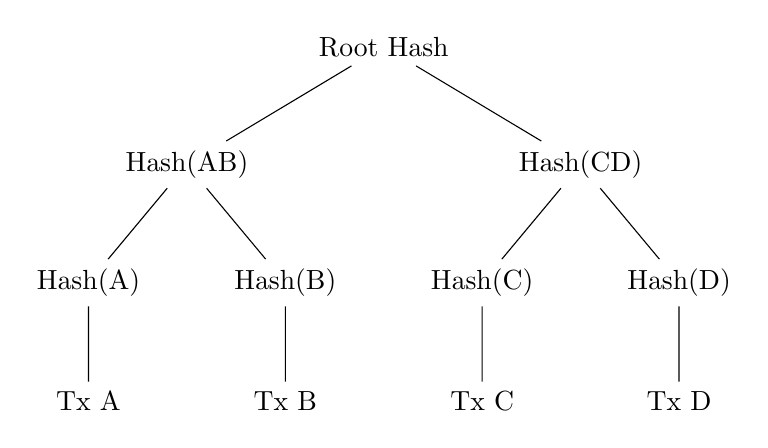
\begin{tikzpicture}[level distance=1.5cm, level 1/.style={sibling distance=5cm}, level 2/.style={sibling distance=2.5cm}]
\node {Root Hash}
    child {node {Hash(AB)}
        child {node {Hash(A)}
            child {node {Tx A}}
        }
        child {node {Hash(B)}
            child {node {Tx B}}
        }
    }
    child {node {Hash(CD)}
        child {node {Hash(C)}
            child {node {Tx C}}
        }
        child {node {Hash(D)}
            child {node {Tx D}}
        }
    };
\end{tikzpicture}
\captionof{figure}{Merkle Tree Creation Example}
\end{center}

\begin{center}
\captionof{table}{Merkle Tree Benefits}
\begin{tabulary}{\linewidth}{|L|L|}
\hline
\textbf{Benefit} & \textbf{Description} \\ \hline
\keyword{Efficiency} & Verify transactions without full data \\ \hline
\keyword{Security} & Any change affects root hash \\ \hline
\keyword{Scalability} & Log(n) verification complexity \\ \hline
\end{tabulary}
\end{center}

\textbf{Verification Process}:

\begin{itemize}
    \item To verify Tx A: Need Hash(B), Hash(CD), and Root Hash
    \item Path verification: Hash(A) + Hash(B) = Hash(AB)
    \item Hash(AB) + Hash(CD) = Root Hash
\end{itemize}

\textbf{Applications}:

\begin{itemize}
    \item \textbf{Bitcoin}: Block headers contain Merkle root
    \item \textbf{SPV Clients}: Light wallets use Merkle proofs
    \item \textbf{Git}: Version control system uses similar structure
\end{itemize}

\begin{mnemonicbox}
\mnemonic{Hash-Pair-Repeat-Root: Merkle Tree Creation Process}
\end{mnemonicbox}
\end{solutionbox}

\questionmarks{4(a) OR}{3}{List various types of Hyperledger projects.}

\begin{solutionbox}
\textbf{Answer}:

\begin{center}
\captionof{table}{Hyperledger Projects}
\begin{tabulary}{\linewidth}{|L|L|L|}
\hline
\textbf{Project} & \textbf{Type} & \textbf{Purpose} \\ \hline
\keyword{Fabric} & Framework & Permissioned blockchain platform \\ \hline
\keyword{Sawtooth} & Framework & Modular blockchain suite \\ \hline
\keyword{Iroha} & Framework & Simple blockchain for mobile/web \\ \hline
\keyword{Burrow} & Framework & Ethereum Virtual Machine \\ \hline
\keyword{Caliper} & Tool & Blockchain performance benchmark \\ \hline
\keyword{Composer} & Tool & Business network development \\ \hline
\end{tabulary}
\end{center}

\textbf{Categories}:

\begin{itemize}
    \item \textbf{Frameworks}: Core blockchain platforms
    \item \textbf{Tools}: Development and testing utilities
\end{itemize}

\begin{mnemonicbox}
\mnemonic{F-S-I-B-C-C: Fabric, Sawtooth, Iroha, Burrow, Caliper, Composer}
\end{mnemonicbox}
\end{solutionbox}

\questionmarks{4(b) OR}{4}{Explain Practical Byzantine Fault Tolerance algorithm in detail.}

\begin{solutionbox}
\textbf{Answer}:

\textbf{Definition}: Consensus algorithm that works correctly even when up to 1/3 of nodes are faulty or malicious.

\begin{center}
\captionof{table}{PBFT Phases}
\begin{tabulary}{\linewidth}{|L|L|L|}
\hline
\textbf{Phase} & \textbf{Description} & \textbf{Purpose} \\ \hline
\keyword{Pre-prepare} & Primary broadcasts request & Initiate consensus \\ \hline
\keyword{Prepare} & Nodes validate and broadcast & Verify proposal \\ \hline
\keyword{Commit} & Nodes commit to decision & Finalize agreement \\ \hline
\end{tabulary}
\end{center}

\textbf{Algorithm Steps}:

\begin{enumerate}
    \item Client sends request to primary replica
    \item Primary broadcasts pre-prepare message
    \item Backups send prepare messages if valid
    \item After receiving 2f+1 prepares, send commit
    \item Execute after receiving 2f+1 commits
\end{enumerate}

\textbf{Key Properties}:

\begin{itemize}
    \item \textbf{Safety}: Never produces inconsistent results
    \item \textbf{Liveness}: Eventually produces results
    \item \textbf{Fault Tolerance}: Works with f < n/3 faulty nodes
\end{itemize}

\begin{mnemonicbox}
\mnemonic{Pre-Prepare-Commit: 3 Phases of PBFT}
\end{mnemonicbox}
\end{solutionbox}

\questionmarks{4(c) OR}{7}{"Eventual consistency is evident in the context of bitcoin." Justify this sentence.}

\begin{solutionbox}
\textbf{Answer}:

\textbf{Definition}: Eventual consistency means the system will become consistent over time, even if it's temporarily inconsistent.

\textbf{Bitcoin Implementation}:

\begin{center}
\captionof{table}{Bitcoin Consistency Mechanisms}
\begin{tabulary}{\linewidth}{|L|L|L|}
\hline
\textbf{Mechanism} & \textbf{Description} & \textbf{Purpose} \\ \hline
\keyword{Chain Reorganization} & Replace shorter chain with longer & Maintain consensus \\ \hline
\keyword{Confirmation Delays} & Wait for multiple blocks & Increase certainty \\ \hline
\keyword{Fork Resolution} & Longest chain wins & Resolve conflicts \\ \hline
\end{tabulary}
\end{center}

\textbf{Scenarios Demonstrating Eventual Consistency}:

\begin{enumerate}
    \item \textbf{Temporary Forks}: When two miners find blocks simultaneously
    \item \textbf{Network Partitions}: Isolated nodes may have different views
    \item \textbf{Double Spending Attempts}: Conflicting transactions in different blocks
\end{enumerate}

\textbf{Resolution Process}:

\begin{itemize}
    \item \textbf{Mining Continues}: Miners build on their preferred chain
    \item \textbf{Longest Chain Rule}: Network adopts chain with most work
    \item \textbf{Automatic Convergence}: All nodes eventually agree
\end{itemize}

\textbf{Diagram: Fork Resolution}

\begin{center}
\begin{tikzpicture}[node distance=2cm, auto, gtu arrow/.style={->, thick}]
    \node [gtu block] (N) {Block N};
    \node [gtu block, right=1.5cm of N] (N1a) {Block N+1a};
    \node [gtu block, above=1cm of N1a] (N1b) {Block N+1b};
    \node [gtu block, right=1.5cm of N1a] (N2a) {Block N+2a};
    \node [gtu block, right=1.5cm of N2a] (main) {Becomes Main Chain};
    \node [gtu block, right=1.5cm of N1b] (die) {Dies - Shorter Chain};

    \draw [gtu arrow] (N) -- (N1a);
    \draw [gtu arrow] (N) -- (N1b);
    \draw [gtu arrow] (N1a) -- (N2a);
    \draw [gtu arrow] (N2a) -- (main);
    \draw [gtu arrow] (N1b) -- (die);
\end{tikzpicture}
\captionof{figure}{Fork Resolution}
\end{center}

\textbf{Justification Points}:

\begin{itemize}
    \item \textbf{Probabilistic Finality}: Longer confirmation time = higher certainty
    \item \textbf{No Immediate Consistency}: New transactions aren't instantly final
    \item \textbf{Convergence Guarantee}: Network will eventually agree on single chain
    \item \textbf{Time-based Resolution}: Consistency improves with time
\end{itemize}

\textbf{Practical Implications}:

\begin{itemize}
    \item \textbf{Merchant Waiting}: Wait for confirmations before accepting payment
    \item \textbf{Exchange Policies}: Different confirmation requirements for different amounts
    \item \textbf{Risk Management}: Balance speed vs security based on transaction value
\end{itemize}

\begin{mnemonicbox}
\mnemonic{Time-Brings-Consistency: Eventual Consistency = Time + Convergence}
\end{mnemonicbox}
\end{solutionbox}

\questionmarks{5(a)}{3}{Explain advantages of ERC 20.}

\begin{solutionbox}
\textbf{Answer}:

\begin{center}
\captionof{table}{ERC-20 Token Advantages}
\begin{tabulary}{\linewidth}{|L|L|}
\hline
\textbf{Advantage} & \textbf{Description} \\ \hline
\keyword{Standardization} & Common interface for all tokens \\ \hline
\keyword{Interoperability} & Works with all Ethereum wallets/exchanges \\ \hline
\keyword{Liquidity} & Easy trading and exchange \\ \hline
\end{tabulary}
\end{center}

\textbf{Key Benefits}:

\begin{itemize}
    \item \textbf{Developer Friendly}: Simple implementation standard
    \item \textbf{Market Adoption}: Widely supported across platforms
    \item \textbf{Smart Contract Integration}: Easy DeFi integration
\end{itemize}

\begin{mnemonicbox}
\mnemonic{SIL: Standard-Interoperable-Liquid}
\end{mnemonicbox}
\end{solutionbox}

\questionmarks{5(b)}{4}{Describe working mechanism of a smart-contract in detail.}

\begin{solutionbox}
\textbf{Answer}:

\begin{center}
\captionof{table}{Smart Contract Workflow}
\begin{tabulary}{\linewidth}{|L|L|}
\hline
\textbf{Step} & \textbf{Description} \\ \hline
\keyword{Code Deployment} & Contract uploaded to blockchain \\ \hline
\keyword{Trigger Conditions} & Predefined conditions monitored \\ \hline
\keyword{Automatic Execution} & Contract executes when conditions met \\ \hline
\keyword{State Update} & Blockchain state modified \\ \hline
\end{tabulary}
\end{center}

\textbf{Working Process}:

\begin{enumerate}
    \item \textbf{Development}: Write contract in Solidity/Vyper
    \item \textbf{Compilation}: Convert to bytecode
    \item \textbf{Deployment}: Upload to blockchain network
    \item \textbf{Execution}: Triggered by transactions or events
\end{enumerate}

\begin{mnemonicbox}
\mnemonic{DTEU: Deploy-Trigger-Execute-Update}
\end{mnemonicbox}
\end{solutionbox}

\questionmarks{5(c)}{7}{What is smart-contract? Explain features and applications of smart-contract in detail.}

\begin{solutionbox}
\textbf{Answer}:

\textbf{Definition}: Self-executing contracts with terms directly written into code, running on blockchain.

\begin{center}
\captionof{table}{Smart Contract Features}
\begin{tabulary}{\linewidth}{|L|L|L|}
\hline
\textbf{Feature} & \textbf{Description} & \textbf{Benefit} \\ \hline
\keyword{Autonomous} & Executes without intermediaries & Cost reduction \\ \hline
\keyword{Transparent} & Code visible on blockchain & Trust building \\ \hline
\keyword{Immutable} & Cannot be changed once deployed & Security \\ \hline
\keyword{Deterministic} & Same input produces same output & Predictability \\ \hline
\end{tabulary}
\end{center}

\textbf{Diagram: Smart Contract Architecture}

\begin{center}
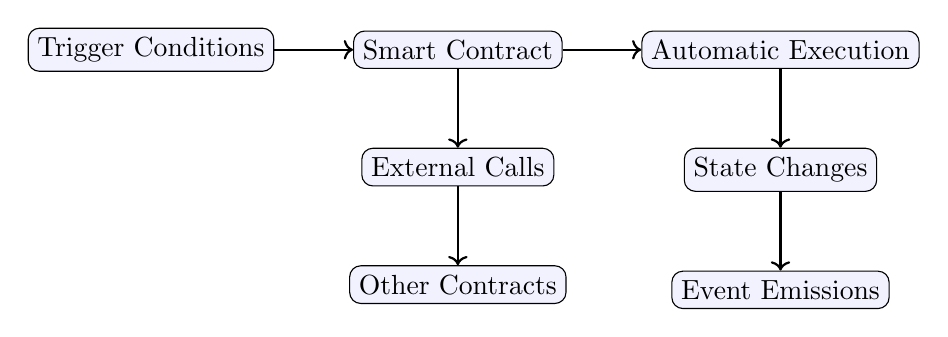
\begin{tikzpicture}[node distance=2.5cm, auto,
    gtu block/.style={rectangle, draw, rounded corners, align=center, fill=blue!5},
    gtu arrow/.style={->, thick}]

    \node [gtu block] (sc) {Smart Contract};
    \node [gtu block, left=1cm of sc] (trigger) {Trigger Conditions};
    \node [gtu block, right=1cm of sc] (exec) {Automatic Execution};
    \node [gtu block, below=1cm of exec] (state) {State Changes};
    \node [gtu block, below=1cm of state] (event) {Event Emissions};
    \node [gtu block, below=1cm of sc] (ext) {External Calls};
    \node [gtu block, below=1cm of ext] (other) {Other Contracts};
    
    \draw [gtu arrow] (trigger) -- (sc);
    \draw [gtu arrow] (sc) -- (exec);
    \draw [gtu arrow] (exec) -- (state);
    \draw [gtu arrow] (state) -- (event);
    \draw [gtu arrow] (sc) -- (ext);
    \draw [gtu arrow] (ext) -- (other);
\end{tikzpicture}
\captionof{figure}{Smart Contract Architecture}
\end{center}

\textbf{Applications}:

\begin{center}
\captionof{table}{Smart Contract Applications}
\begin{tabulary}{\linewidth}{|L|L|L|}
\hline
\textbf{Domain} & \textbf{Use Case} & \textbf{Example} \\ \hline
\keyword{Finance} & Automated lending & DeFi protocols \\ \hline
\keyword{Insurance} & Claim processing & Flight delay insurance \\ \hline
\keyword{Supply Chain} & Product tracking & Food provenance \\ \hline
\keyword{Real Estate} & Property transfers & Automated escrow \\ \hline
\keyword{Gaming} & Digital assets & NFT marketplaces \\ \hline
\end{tabulary}
\end{center}

\textbf{Advantages}:

\begin{itemize}
    \item \textbf{Efficiency}: Reduced processing time and costs
    \item \textbf{Trust}: No need for trusted third parties
    \item \textbf{Accuracy}: Eliminates human errors
    \item \textbf{Global Access}: Available 24/7 worldwide
\end{itemize}

\textbf{Limitations}:

\begin{itemize}
    \item \textbf{Immutability}: Difficult to fix bugs after deployment
    \item \textbf{Oracle Problem}: Need external data sources
    \item \textbf{Gas Costs}: Execution costs can be high
    \item \textbf{Complexity}: Requires technical expertise
\end{itemize}

\textbf{Development Considerations}:

\begin{itemize}
    \item \textbf{Security Audits}: Essential before deployment
    \item \textbf{Testing}: Extensive testing on testnets
    \item \textbf{Upgradability}: Design patterns for updates
    \item \textbf{Gas Optimization}: Minimize execution costs
\end{itemize}

\begin{mnemonicbox}
\mnemonic{ATID: Auto-Transparent-Immutable-Deterministic}
\end{mnemonicbox}
\end{solutionbox}

\questionmarks{5(a) OR}{3}{Explain disadvantages of ERC20.}

\begin{solutionbox}
\textbf{Answer}:

\begin{center}
\captionof{table}{ERC-20 Token Disadvantages}
\begin{tabulary}{\linewidth}{|L|L|}
\hline
\textbf{Disadvantage} & \textbf{Description} \\ \hline
\keyword{Limited Functionality} & Only basic token operations \\ \hline
\keyword{No Built-in Security} & Vulnerable to common attacks \\ \hline
\keyword{Gas Dependency} & Requires ETH for transactions \\ \hline
\end{tabulary}
\end{center}

\textbf{Key Issues}:

\begin{itemize}
    \item \textbf{Transfer Limitations}: Cannot handle complex transfers
    \item \textbf{Approval Risks}: Double spending vulnerabilities
    \item \textbf{Network Congestion}: High fees during peak times
\end{itemize}

\begin{mnemonicbox}
\mnemonic{LVD: Limited-Vulnerable-Dependent}
\end{mnemonicbox}
\end{solutionbox}

\questionmarks{5(b) OR}{4}{Describe steps for Launching of a Decentralized Autonomous Organization (DAO)?}

\begin{solutionbox}
\textbf{Answer}:

\begin{center}
\captionof{table}{DAO Launch Steps}
\begin{tabulary}{\linewidth}{|L|L|}
\hline
\textbf{Step} & \textbf{Description} \\ \hline
\keyword{Concept Design} & Define purpose and governance rules \\ \hline
\keyword{Smart Contract Development} & Code governance mechanisms \\ \hline
\keyword{Token Distribution} & Allocate voting rights \\ \hline
\keyword{Community Building} & Attract members and contributors \\ \hline
\end{tabulary}
\end{center}

\textbf{Detailed Process}:

\begin{enumerate}
    \item \textbf{Whitepaper Creation}: Document vision and tokenomics
    \item \textbf{Technical Implementation}: Deploy governance contracts
    \item \textbf{Initial Funding}: Raise capital through token sales
    \item \textbf{Operations Launch}: Begin decentralized operations
\end{enumerate}

\begin{mnemonicbox}
\mnemonic{4D Launch: Design-Develop-Distribute-Deploy}
\end{mnemonicbox}
\end{solutionbox}

\questionmarks{5(c) OR}{7}{What is Decentralized Autonomous Organization (DAO)? Explain its advantages and disadvantages in detail.}

\begin{solutionbox}
\textbf{Answer}:

\textbf{Definition}: A blockchain-based organization governed by smart contracts and token holders rather than traditional management.

\begin{center}
\captionof{table}{DAO Structure}
\begin{tabulary}{\linewidth}{|L|L|L|}
\hline
\textbf{Component} & \textbf{Description} & \textbf{Function} \\ \hline
\keyword{Smart Contracts} & Governance rules in code & Automated decision execution \\ \hline
\keyword{Tokens} & Voting rights and ownership & Democratic participation \\ \hline
\keyword{Proposals} & Suggested changes or actions & Community-driven initiatives \\ \hline
\keyword{Treasury} & Shared funds & Resource allocation \\ \hline
\end{tabulary}
\end{center}

\textbf{Diagram: DAO Governance Flow}

\begin{center}
\begin{tikzpicture}[node distance=2cm, auto, gtu arrow/.style={->, thick}]
    \node [gtu block] (holders) {Token Holders};
    \node [gtu block, right=1.5cm of holders] (proposals) {Submit Proposals};
    \node [gtu block, below=1cm of proposals] (discussion) {Community Discussion};
    \node [gtu block, left=1.5cm of discussion] (voting) {Voting Period};
    \node [gtu block, below=1cm of voting] (execution) {Execution if Passed};
    \node [gtu block, right=1.5cm of execution] (updates) {Smart Contract Updates};
    \node [gtu block, below=1cm of updates] (treasury) {Treasury Actions};
    
    \draw [gtu arrow] (holders) -- (proposals);
    \draw [gtu arrow] (proposals) -- (discussion);
    \draw [gtu arrow] (discussion) -- (voting);
    \draw [gtu arrow] (voting) -- (execution);
    \draw [gtu arrow] (execution) -- (updates);
    \draw [gtu arrow] (updates) -- (treasury);
\end{tikzpicture}
\captionof{figure}{DAO Governance Flow}
\end{center}

\textbf{Advantages}:

\begin{center}
\captionof{table}{DAO Benefits}
\begin{tabulary}{\linewidth}{|L|L|L|}
\hline
\textbf{Advantage} & \textbf{Description} & \textbf{Impact} \\ \hline
\keyword{Decentralization} & No single point of control & Reduced corruption risk \\ \hline
\keyword{Transparency} & All decisions on blockchain & Enhanced accountability \\ \hline
\keyword{Global Participation} & Anyone can join & Diverse perspectives \\ \hline
\keyword{Efficiency} & Automated execution & Faster decision implementation \\ \hline
\keyword{Democratic Governance} & Token-based voting & Fair representation \\ \hline
\end{tabulary}
\end{center}

\textbf{Disadvantages}:

\begin{center}
\captionof{table}{DAO Challenges}
\begin{tabulary}{\linewidth}{|L|L|L|}
\hline
\textbf{Disadvantage} & \textbf{Description} & \textbf{Risk} \\ \hline
\keyword{Technical Complexity} & Smart contract bugs & System failures \\ \hline
\keyword{Legal Uncertainty} & Unclear regulatory status & Compliance issues \\ \hline
\keyword{Coordination Problems} & Difficult decision making & Slow progress \\ \hline
\keyword{Token Concentration} & Wealthy holders control votes & Centralization risk \\ \hline
\keyword{Security Vulnerabilities} & Code exploits possible & Financial losses \\ \hline
\end{tabulary}
\end{center}

\textbf{Types of DAOs}:

\begin{itemize}
    \item \textbf{Investment DAOs}: Collective investment decisions
    \item \textbf{Protocol DAOs}: Blockchain protocol governance
    \item \textbf{Social DAOs}: Community-driven organizations
    \item \textbf{Collector DAOs}: NFT and art collecting
\end{itemize}

\textbf{Success Factors}:

\begin{itemize}
    \item \textbf{Clear Purpose}: Well-defined mission and goals
    \item \textbf{Robust Governance}: Effective voting mechanisms
    \item \textbf{Community Engagement}: Active member participation
    \item \textbf{Technical Security}: Audited smart contracts
    \item \textbf{Legal Compliance}: Regulatory compliance where applicable
\end{itemize}

\textbf{Notable Examples}:

\begin{itemize}
    \item \textbf{MakerDAO}: Decentralized finance protocol
    \item \textbf{Uniswap}: Decentralized exchange governance
    \item \textbf{Compound}: Money market protocol
\end{itemize}

\textbf{Future Outlook}:

\begin{itemize}
    \item \textbf{Regulatory Clarity}: Evolving legal frameworks
    \item \textbf{Technical Improvements}: Better governance tools
    \item \textbf{Mainstream Adoption}: Growing corporate interest
    \item \textbf{Integration}: Hybrid traditional-DAO models
\end{itemize}

\begin{mnemonicbox}
\mnemonic{DAO: Democratic Automated Ownership}
\end{mnemonicbox}
\end{solutionbox}

\end{document}
